\documentclass{beamer}
\usepackage[ngerman]{babel}
\usepackage{graphicx}
\usepackage{subfiles}


\graphicspath{{resources/}}

\beamertemplatenavigationsymbolsempty

\usetheme[noflama]{custom}

\title{Funktionale \break Programierung}
\subtitle{Nebenläufigkeit \& Parallelisierung}
\author{Jan-Philipp Willem}
\institute{
  Hochschule Mannheim\\
  Fakultät für Informatik\\
  Prof. Dr. Sandro Leuchter
}
\date{Seminar, WS2016}

\begin{document}

\begin{frame}[noframenumbering,plain]
  \frametitle{Was wird hier gezeigt?}
  \centering
  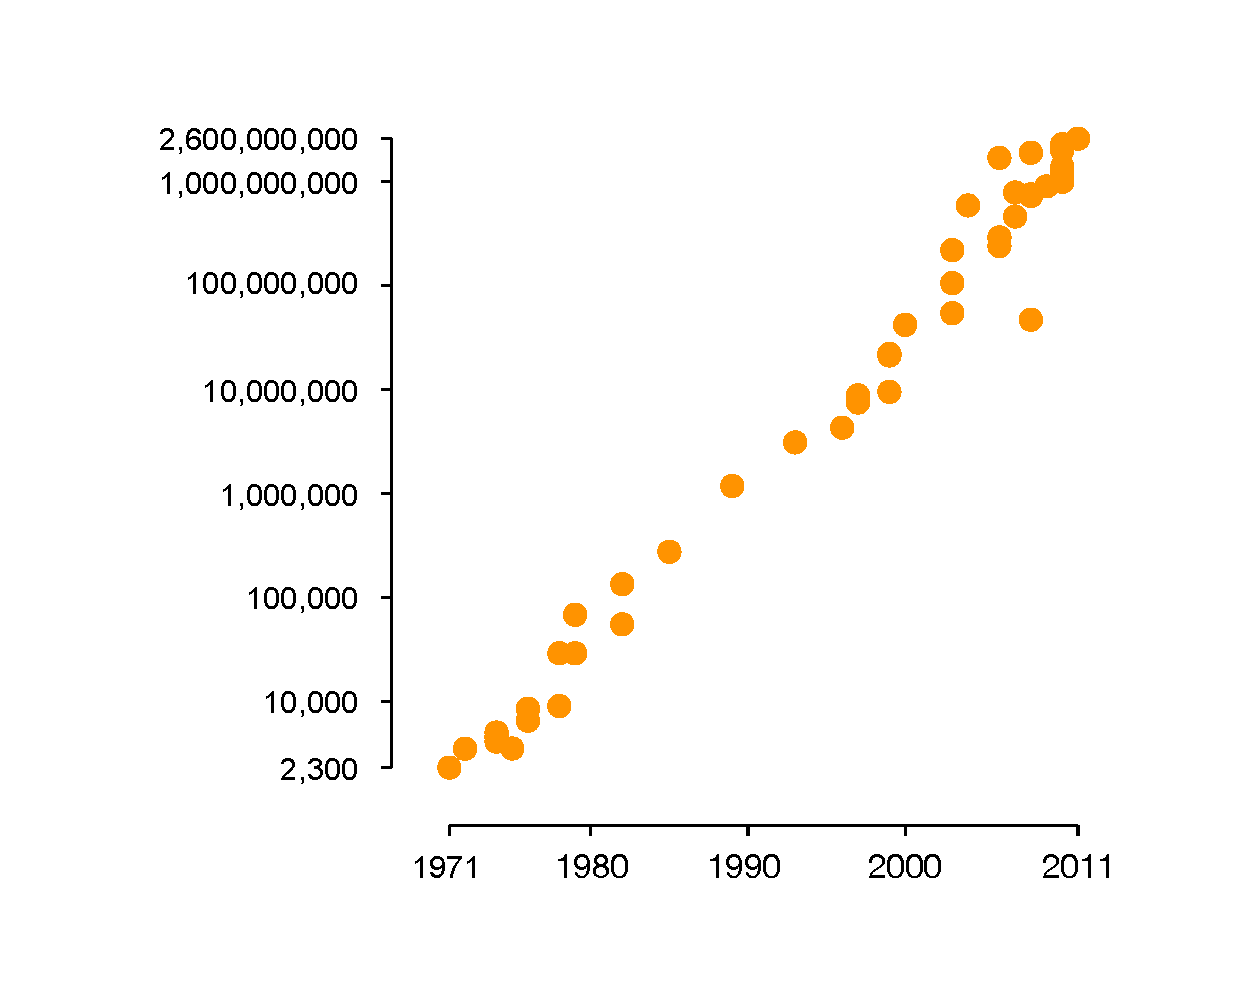
\includegraphics[width=0.9\textwidth]{moores_law.pdf}
\end{frame}
 
\begin{frame}[noframenumbering,plain]
  \frametitle{Transistor Counts 1971-2011 \& Moore's Law}
  \centering
  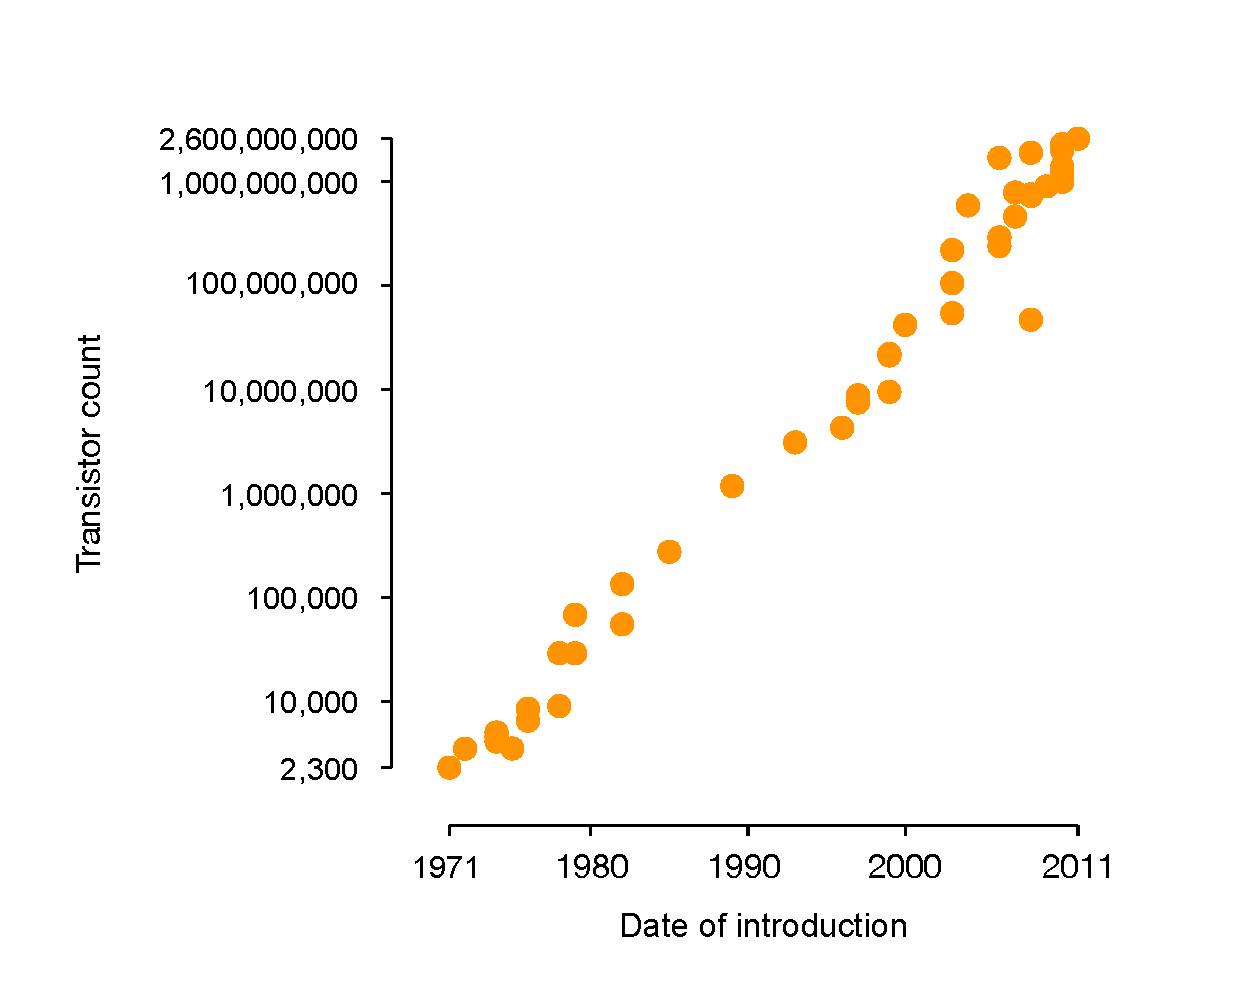
\includegraphics[width=0.9\textwidth]{moores_law_with-labels.pdf}
\end{frame}

\maketitle

\section*{Gliederung}
\begin{frame}[noframenumbering,plain]{Gliederung}
  \tableofcontents[hideallsubsections]
\end{frame}

\note[itemize]{
    \item The audience sees the slides, but you see your notes.
    \bigskip
    \item Or, if your don't have notes, you can use mirror mode.
}


\section[Bla]{Bla}
\begin{frame}{Sample frame title}
\setcounter{framenumber}{1}
  This is a text in first frame. This is a text in first frame. This is a text in first frame.
\end{frame}

\section[Foo]{Foo}
\begin{frame}{Sample frame title}
  This is a text in first frame. This is a text in first frame. This is a text in first frame.
\end{frame}
\end{document}
